% =============================================================================
% midcenturymodern_demo.tex
% Demo file for the Mid-Century Modern Beamer template.
% Compile with: lualatex midcenturymodern_demo.tex
% =============================================================================
% !TeX program = LuaLaTex
\documentclass[aspectratio=169]{beamer}
\usepackage{beamerthememidcenturymodern}
\usepackage{svg}
\usepackage[backend=biber, style=authoryear, sorting=nyt]{biblatex}
\addbibresource{demo.bib}

% --- Theme selection (comment/uncomment to switch) ---
\mcmTheme{DeepBlue}
% \mcmTheme{DeepBlue}
 % 
% --- Metadata ---
\title{In Search of Calabi-Yau 3-Folds}
\subtitle{Moduli Space of $n_3$ Configurations}
\author{Henry Morin}
\institute{Under the Supervision of Jenia Tevelev}
\date{July 24, 2026}


\titlegraphic{
  \begin{minipage}{0.21\linewidth}
    \begin{center}
    
\includegraphics[width=1.7cm]{images/UMassSeal.png}
    % \includegraphics[width=3cm]{logos/logo_deepblue.png}
    \end{center}
  \end{minipage}
}

% --- Automatic section/subsection pages ---
\AtBeginSection[]{%
  \begin{frame}[plain]
    \sectionpage
  \end{frame}
}
\AtBeginSubsection[]{%
  \begin{frame}[plain]
    \subsectionpage
  \end{frame}
}

\AtEveryCite{\color{mcmPrimary}}

\begin{document}

% =====================================================================
% TITLE PAGE
% =====================================================================
\begin{frame}
  \titlepage
\end{frame}

% =====================================================================
% TABLE OF CONTENTS
% =====================================================================
%
% =====================================================================
\section{Calabi-Yau Manifolds}
% =====================================================================


\begin{frame}{Manifolds}
      \begin{block}{Definition}
        \begin{itemize}
            \item "Nice" subsets of $\mathbb{R}^N$
            \item Locally flat, that is locally $\mathbb{R}^d$
          \item Classical object of study in physics and mathematics
        \end{itemize}
    \end{block}
\end{frame}

\begin{frame}{Manifolds}
        \begin{block}{Examples}
            \begin{itemize}
                \item Open subsets of $\mathbb{R}^N$
                \item Spheres
                \item Tori
                \item Projective Space ($\mathbb{P}^n$)
            \end{itemize}
        \end{block}
\end{frame}


\begin{frame}{Calabi-Yau Manifolds}
    \begin{block}{Definition}
        \begin{itemize}
            \item Globally "flat" manifolds $M$
            \item Even dimensional $2d$
            \item Trivial Canonical Line Bundle $\omega_M = \bigwedge^{2d}T^{\ast}M = 0$
        \end{itemize}
    \end{block}
\end{frame}

\begin{frame}{Calabi-Yau Manifolds}
    \begin{columns}[T]
        \begin{column}{0.48\linewidth}
        \begin{block}{Examples}
            \begin{itemize}
            \item Elliptic curves (complex tori)
            \item Smooth $4$-dimensional quartic surfaces
            \item Smooth $6$-dimensional quintic surfaces
        \end{itemize}
        \end{block}
    \end{column}
    \begin{column}{0.48\linewidth}
        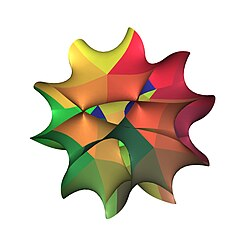
\includegraphics[width = 0.9\textwidth]{images/CalabiYau5.jpg}
    \end{column}
\end{columns}
\end{frame}


\begin{frame}{Calabi-Yau Manifolds}
    \begin{block}{Why do we Care?}
        \begin{itemize}
            \item CY manifolds naturally arise in physics
            \item Classification of CY manifolds important in string theory 
            \item CY manifolds are interesting in their own right
        \end{itemize}
    \end{block}
\end{frame}

  
\begin{frame}{Construction}
    \begin{block}{General Method}
        \begin{itemize}
            \item Degree $n + 1$ polynomial equation in $n$ variables $f$
            \item Take $Z(f) := \{z \in \mathbb{C}^n \mid f(z) = 0\}$
            \item Add points at $\infty$
            \item Desinguralize
        \end{itemize}
    \end{block}
\end{frame}

\begin{frame}{Problem}
    \begin{block}{This is Hard}
        \begin{itemize}
            \item Very difficult to obtain $f$ of higher degree
            \item Once you have $f$, desinguralization can be expensive
            \item "Shape Shift" - Admit many models
        \end{itemize}
    \end{block}
\end{frame}

\section{$n_3$ Configurations}
\begin{frame}{$n_3$ Configurations}
    \begin{columns}[T]
        \begin{column}{0.48\linewidth}
    \begin{block}{Definition}
        \begin{itemize}
            \item "Points" $P = \{1,\dots,n\}$ 
            \item "Lines" $L \subset 2^P$
        \item $n_3$ condition: $|\ell| = 3$ and $|\{\ell \mid i \in \ell\}| = 3$
        \end{itemize}
    \end{block}
    \end{column}
    \begin{column}{0.48\linewidth}
        \begin{tabular}{c | c}
                $n$ &  $n_3$ configurations \\
                \hline
                $7$ & $1$ \\
                $8$ & $1$ \\
                $9$ & $3$ \\
                $10$ & $10$ \\
                $11$ & $31$ \\
                $12$ & $229$ \\
                $13$ & $2036$ \\
        \end{tabular}
    \end{column}
\end{columns}
\end{frame}

\begin{frame}{$n_3$ Moduli Spaces}
    \begin{block}{Definition}
        \begin{itemize}
            \item Fix $n_3$ configuration $(P, L)$
            \item A \textbf{moduli space} is the set $M$ of solutions to a polynomial 
            \item Such that $z \in M$ corresponds to one way of drawing $(P, L)$
        \end{itemize}
    \end{block}
\end{frame}


\begin{frame}{Adjunction Computation}
    \begin{block}{Setup}
        \begin{itemize}
            \item $M$ is given by the set of points $(p_1, p_2,\dots, p_n) \in (\mathbb{P}^2)^n$
            \item Such that $p_i,p_j,p_k$ are collinear in $\mathbb{P}^2$ iff $i,j,k \in \ell$ for some $\ell \in L$.
            \item Given by $n$ equations of multi-degrees $(0,\dots,1,1,1,\dots,0)$
            \item Successively applying the restrictions we obtain 
                \[M \subset M_{n - 1} \subset M_{n - 2} \subset \cdots \subset M_{1} \subset (\mathbb{P}^2)^n\]
            \item Quotient by $\text{PGL}(3)$
        \end{itemize}
    \end{block}
\end{frame}

\begin{frame}{Adjunction Computation}
    \begin{block}{Computing $\omega_M$}
        \begin{itemize}
            \item Canonical class $\omega$ of a hypersurface is given as $\iota^* (\omega \otimes \mathcal{O}(d))$
            \item $\omega_{M_1} = \iota^\ast(\omega_{(\mathbb{P}^2)^n} \otimes \mathcal{O}((1,1,1,0,\dots,0)))$
        \end{itemize}
        \begin{align*}
            \omega_{M_1} &= \iota^\ast(\omega_{(\mathbb{P}^2)^n} \otimes \mathcal{O}((1,1,1,0,\dots,0))) \\
            \omega_{M_2} &= \iota^\ast(\omega_{M_1} \otimes \mathcal{O}((1,0,1,1,0\dots,0))) \\
            \vdots &\hspace{40mm} \vdots \\
            \omega_{M} &= \iota^\ast(\omega_{M_{n-1}} \otimes((0,0,\dots,0,1,1,1)))
        \end{align*}
    \end{block}
\end{frame}

\begin{frame}{Adjunction Computation}
    \begin{block}{$M$ is Calabi-Yau!}
        \begin{itemize}
            \item Since $\omega_{(\mathbb{P}^2)^n} = \mathcal{O}(-3,-3\dots,-3)$
            \item This becomes (by omitting $\mathcal{O}$):
        \end{itemize}
        \begin{align*}
            (-2,-2,-2,-3,\dots,-3) &= \iota^\ast((-3,-3,\dots,-3) \otimes (1,1,1,0,\dots,0)) \\
            (-1,-2,-1,-2,\dots,-3) &=  \iota^\ast((-2,-2,-2,-3,\dots,-3) \otimes (1,0,1,1,0\dots,0)) \\
            \vdots &\hspace{40mm} \vdots \\
            (0,0,\dots,0) &= \iota^\ast((0,0,\dots,0,-1,-1,-1) \otimes (0,0,\dots,0,1,1,1))
        \end{align*}

        So $\omega_M = 0$!
    \end{block}
\end{frame}

\begin{frame}{$n = 7$}
    \begin{columns}[T]
        \begin{column}{0.48\linewidth}
    \begin{block}{Summary}
        \begin{itemize}
            \item Number of configurations: $1$ (Fano Plane)
            \item Moduli Space: $f = 1$
            \item Not realizable in $\text{char} \ne 2$
        \end{itemize}
    \end{block}
    \end{column}
    \begin{column}{0.48\linewidth}
        \hspace{10mm}
        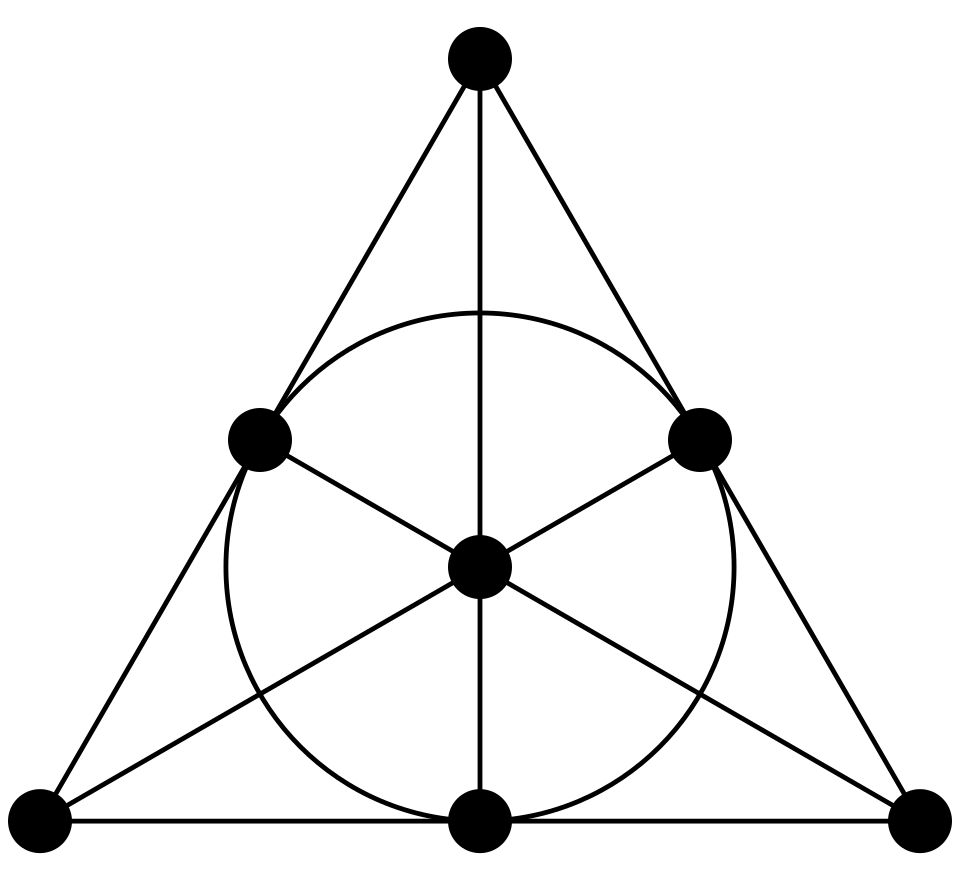
\includegraphics[width = 0.6\linewidth]{images/Fano_Planepng.png}
    \end{column}
\end{columns}
\end{frame}

\begin{frame}{$n = 8$}
    \begin{columns}[T]
        \begin{column}{0.48\linewidth}
    \begin{block}{Summary}
        \begin{itemize}
            \item Number of configurations: $1$ (M\"{o}bius Cantor Configuration)
            \item Moduli Space: $f = x^2 - x + 1$
            \item 2 realizations corresponding to
        \end{itemize}
        \[x = \frac{1 \pm \sqrt{-3}}{2}\]
    \end{block}
\end{column}
\begin{column}{0.48\linewidth}
    \hspace{5mm}
    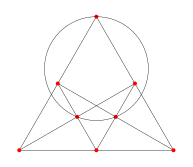
\includegraphics[width = 0.70\linewidth]{images/MKConfig1000.png}
\end{column}
\end{columns}
\end{frame}

\begin{frame}{$n = 9$}
    \begin{columns}[T]
    \begin{column}{0.48\linewidth}
    \begin{block}{Summary}
        \begin{itemize}
            \item Number of configurations: $3$
            \item Moduli Spaces: $f = 0$
            \item One "wrong" dimension (Pappus Configuration)
        \end{itemize}
    \end{block}
\end{column}
\begin{column}{0.48\linewidth}
    \hspace{10mm}
    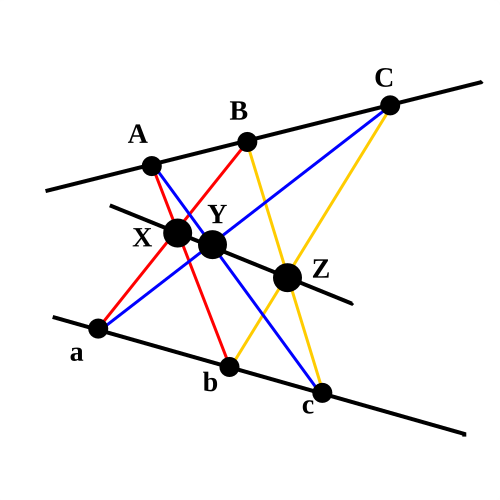
\includegraphics[width = 0.60\linewidth]{images/Pappusconfig.png}
\end{column}
\end{columns}
\end{frame}


\begin{frame}{$n = 10$ (Elias Sink)}
    \begin{columns}[T]
        \begin{column}{0.48\linewidth}
            \begin{itemize}
                \item Number of configurations: $10$
                \item One not realizable in any characteristic
                \item Moduli Spaces: Four are $K3$ surfaces, five are given by $f = 0$
                \item One "wrong" dimension (Desargues Configuration)
            \end{itemize}
        \end{column}
        \begin{column}{0.48\linewidth}
            \hspace{10mm}
            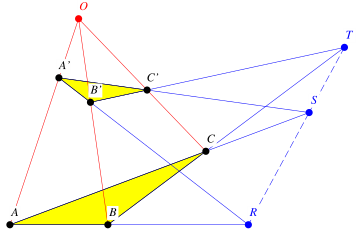
\includegraphics[width = 0.70\linewidth]{images/DesarguesTheorem.png}
        \end{column}
    \end{columns}
\end{frame}



\begin{frame}{$n = 11$ (Current Research)}
    \begin{block}{Summary}
        \begin{itemize}
            \item Number of configurations: $31$
            \item 7 known to be given by $f = 0$, 12 quintic, 5 sextics, 3 septics, 4 octics
            \item We currently are working towards desinguralization of quintic examples
            \item We have three (non confirmed) Calabi-Yau matches
        \end{itemize}
    \end{block}
\end{frame}

\begin{frame}{Future Directions}
    \begin{block}{Ongoing Work}
        \begin{itemize}
            \item Analyse double cover models by blowups of $\mathbb{P}^3$ 
            \item Utilize $K3$ fibration structure on $M$ to obtain smooth model
            \item Utilize elliptic fibration structure on $M$ to obtain smooth model
            \item Study rigidity of $M$
            \item Study modularity of $M$
        \end{itemize}
    \end{block}
\end{frame}

\begin{frame}{Sources}
    \begin{itemize}
        \item E. Sink, Line Configurations and K3 Surfaces. https://arxiv.org/abs/2312.07542
        \item C. Myer, Modular Calabi-Yau Threefolds. https://www.ams.org/books/fim/022/fim022-endmatter.pdf
    \end{itemize}
\end{frame}

\end{document}
